% !TeX root = ..\..\main.tex
\chapter{Introduction}
\pagenumbering{arabic}
This report studies a vital financial derivative in today's markets, namely options. The importance of the option market has been shown by empirical studies which suggest that option trading improves information efficiency in the broader stock market~\cite{PanInfoEffic,li2021effect}, and also that firms with listed options experience lower implied cost of equity capital~\cite{naikerLowEquity}; indicating that options trading reduces the cost of capital~\cite{li2021effect}. The popularity of the options market can easily be seen in \autoref{C1fig:OptionVolume}, which shows the exponential growth in trading volume since standardized, exchange-traded stock options were first listed in The Chicago Board Options Exchange in 1973~\cite{markham2002financial}. In 2020 single stock option trading volume became higher than the underlying stock volume for the first time ever~\cite{yahooOptions}. 
\nline{}
It is this explosive popularity and significance which have motivated this report. 
\\\\
We will begin by describing standard options and explore popular methods that are used to price them. We will then move onto Asian options and look at the literature surrounding how to price them before implementing several pricing methods with the use of \textsc{Matlab}. Furthermore, we will then take an analytical approach to determine how Asian options can be priced accurately and efficiently.
\\\\

\begin{figure}[H]
    \centering
    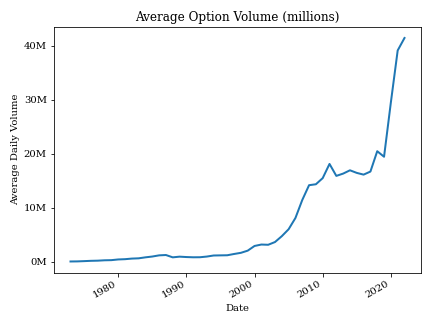
\includegraphics[width=\sOneSize\textwidth]{Chapters/C1/plots/OptionVolume.png}
    \caption{Time series plot of the average daily option trading volume per annum. Data from by the Options Clearing Corporation (OCC)~\cite{THEOCC}. Source code: \autoref{ApPy:lst option volume plot}}\label{C1fig:OptionVolume}\end{figure}

\section{A brief overview of call and put options}

Options are a particular type of financial derivative, a contract that details the conditions under which payments are made between two counterparties. They are purchased for a set fee, and in return the buyer is granted the right, but not the obligation, to buy or sell an underlying asset --- such as commodities, stocks or bonds --- for a predetermined price (the strike price) on or before a determined date (the expiry date).
\nline{}
Call options allow the buyer to purchase an asset for the strike price at a future date. The buyer can make a return if the value of the asset is worth more than the strike price when exercised. Alternatively, put options allow the buyer to sell an asset for the strike price at a future date and the buyer can make a return if the value of the asset is less than the strike price when exercised.
\nline{}
The option market is widely considered a venue for informed trading~\cite{li2021effect,hu2014,chak2004}, that is, investors trading with superior knowledge of the probability distribution of share prices, through either access to private information or skilful processing of public information~\cite{grossman1975application}. 

\subsection{A short history of option trading}
The history of financial options can be traced as far back as 6th century BCE when ancient Greek mathematician and philosopher Thales of Miletus predicted through his astrological knowledge there was going to be a great olive harvest. As he did not have much money, he used what he had as a deposit on the rights to the local olive presses; due to no competition he secured this at a relatively low price. When the harvest proved to be bountiful leading to high demand, Thales charged a high price for use of the presses and reaped a considerable profit. His deposit gave him the right but not the obligation to hire the presses, thus his losses were limited to his initial deposit~\cite{OptionFirst, 1877aristotle}.
\nline{}
Whilst this is quite a positive look on option trading, throughout history this has not always been the case. During the Dutch tulip bubble of the seventeenth century, tulips were seen as a status symbol which caused high demand and consequently drove their prices up, creating a bubble~\cite{dash2011tulipomania}. Tulip growers would buy puts to protect their profits in case the price of tulip bulbs went down and wholesalers would buy calls to protect against the risk of tulip bulbs going up. When the bubble eventually burst, there was no way to force investors to fulfil their obligations under the options contract, due to the unregulated nature of the option market. This ultimately led to options gaining a dubious reputation and bans were later placed on them within Britain between 1733--1860~\cite{OptionBan}. 
\nline{}
During the late nineteenth century, brokers started to arrange deals between buyers and sellers of options for particular stocks at prices that were arranged between the two parties. Trades were arranged similarly until the 1960s when the options market started to become regulated by the Chicago Board of Trade. In 1973, the Chicago Board of Options Exchange (CBOE) began trading and for the first time options contracts were properly standardized. At the same time, the Options Clearing Corporation was established for centralized clearing and enforcing the proper fulfilment of contracts, ensuring that they were honoured~\cite{markham2002financial}.

\subsection{Standard options}

A standard option comes in two styles; European: which restricts the holder of the option to only exercise the option on the expiry date, and American: which allows the holder to exercise the option at anytime up till or on the expiry date. They will take the current value of the underlying asset as the spot price --- that is the price that the asset can be purchased for on the open market. The payoff in this case then becomes the difference between the spot price and strike price.
\nline{}
Mathematically we write the payoff \(\poff{t}\) of a European put option with strike price \(E\), expiry date \(T\) and underlying asset price at time \(t\) being \(S\p{t}\):

\begin{equation*}
    \poff{T} = \max\p{E-S(T),0} 
\end{equation*}

and similarly for a European call option

\begin{equation*}
    \poff{T} = \max\p{S(T)-E,0}
\end{equation*}

An American put or call option payoff is identical however it may be exercises at anytime up to the expiry date, giving: \(\poff{t} \quad \forall t \in [0,T]\).

\subsection{Asian options}

Whilst standard options involve using the spot price as the underlying value of the asset; this is not always the case with so-called exotic options. Exotic options differ in their payment structures, expiration dates, and/or strike prices. In the case of exotic fixed-strike price Asian options, the average price of the asset is used in place of the underlying asset value. This differs from fixed-price Asian options which instead use the average price of the asset to take place of the strike price. These are the two main variations of Asian style options but both of these can be varied further in how the averaging is calculated, for example: geometrically, arithmetically, average taken every day or average taken at the start of each month and so on. They can be varied further by having an expiry structure matching a European or American style option.
\nline{}
A fixed-strike price Asian option with strike price \(E \), expiry time \(T \) and underlying asset value at time \(t\) being \(S(t)\); has the following put and call payoff functions \(\poff{t}\):

\begin{align*}
    \poff{t} = \max\p{E-f\p{t,\delta t},\;0} && \poff{t} = \max\p{f\p{t,\delta t}-E,\;0}
\end{align*}


For some averaging function \(f(t,\delta t)\) where \(\delta t\) represents the time increment for which the average is calculated upon. For an arithmetic average taken every day when time, \(t\) units is days our averaging function is:

\begin{equation*}
    f\p{t,\delta t} = \p{\left\lfloor\frac{t}{\delta t}\right\rfloor}^{-1} \sum_{i=0}^{\lfloor t/\delta t\rfloor}S(i\delta t)
\end{equation*}

Note that \(\forall x\in\rel \; \lfloor x \rfloor \) notation represents the greatest integer less than or equal to \(x \). This allows the function to work for early exercise when \(t\in[0,T] \) in the case of American type Asian options.

\section{Market definition and assumptions}

To begin pricing options we must first establish assumptions on the value of assets and the market in which they are traded. We will consider a market in which there are two classes of assets; risk-free assets and risky assets. We allow derivatives to exist on risky assets.

\subsection{Asset definitions}

We define our two classes of assets with the following assumptions:

\subsubsection{Risk-free assets}

Risk-free assets are assumed to have no uncertainty in regard to their future value and defined as returning interest continuously compounded at a fixed rate \(r\). Hence, an investment of \(A\) made at time \(t\) will return \(A^{r\left(T-t\right)}\) at time \(T>t\) with no uncertainty. These can be positive e.g., making an investment, or negative e.g., taking out a loan. Risk-free assets are akin to fixed rate investments at a well-know bank or government bonds. However, even sovereign nations have been known to default on their bond repayments so in reality are not truly risk-free, but instead considered low-risk~\cite{kitanov2015risk}.

\subsubsection{Risky assets}

Risky assets are assets in which the future value can not be determined without at least some uncertainty. These are typically shares in a company or commodities such as gold and oil. These assets are traded on the open market and their value is heavily dependent on the balance of supply and demand of the asset; this in turn is dependent on so many variables that we assume their future value to be a random process. Depending on our model we can make different assumptions on the distribution of this process and thus how the value evolves over a time period. In practice has been arguments made for the future value of risky assets are truly random~\cite{RandomWalkFama}, and other arguments that propose they are instead at least partly deterministic where patterns and trends exists~\cite{shiller}.

\subsection{Market Assumptions}

We shall assume that an investor may hold any quantity (including negative and/or fractional) of an asset, known as the \textit{divisibility} and \textit{short-selling} assumption. We will also assume that our market is \textit{frictionless} --- that is that any quantity of assets can be bought and sold at the same price with no transaction cost and are entirely \textit{liquid} meaning there is always a buyer for every seller and vice versa.
\nline{}
In practice these assumptions do not accurately represent real markets, for example it is common place for markets to have bid-ask spreads which represents the different in price at which you can buy and sell assets. Furthermore, transaction costs are impossible to fully eliminate --- even in scenarios with no tax or commission fees, buying or selling assets (especially in large quantities) will in theory have an effect on the supply and demand of that asset; this introduces market impact costs~\cite{moro2009market}. There are other transaction fees to also consider such as: time spent deciding what assets to buy, computing power costs and their associated opportunity costs.

\subsubsection{No-Arbitrage assumption}\label{subsubsec: No Arb}

Perhaps our most important market assumption is the No-Arbitrage principle; sometimes referred to as the no free-lunch principle. This assumption states that there can be no risk-free way to get a better rate of return than the market risk-free interest rate, \(r\). The logic behind this assumption is that if there exists a way to earn a higher rate of return than \(r\) with no initial outlay; than other traders would employ the same method and market forces would eliminate the arbitrage opportunity. This assumption assumes that markets are perfectly efficient meaning all traders have access to the same information and that market adjustments to supply and demand happen instantaneously, which we know not to be true in practice.

\section{Asset pricing models}

Having now established our market assumptions, we must now define our assumptions on the random process which describes how the asset value may evolve over a specified time period. We will first introduce the mathematical concepts on which these models are built upon. Then we will introduce a simple asset model and one which has more assumptions in hopes of better describing the future asset value in practice.

\subsubsection{Stochastic processes}

A stochastic process is defined as a collection of random variables defined on a common probability space \( (\Omega ,\mathcal{F},P) \), where \( \Omega \)  is a sample space, \( \mathcal{F} \) is a \( \sigma \)-algebra, and \( P \) is a probability measure; and the random variables, indexed by some set \( T \), all take values in the same mathematical space \(S\), which must be measurable with respect to some \( \sigma \)-algebra \( \Sigma \)~\cite{lamperti1977stochastic}.
\nline{}
A discrete stochastic process is a sequence of random variables which represent observations taken at discrete times from a random system, e.g.\ observations \( \{X_i\,:\, i \in \nat_{[0,n]}\} \) at times \( t = t_0,t_1,\,\dots \,t_n \). We can let our market be the random system and our observations, \( X_i \) be the value of our asset observed on the \( i^\text{th}\) day. This is a typical example of structuring an asset market as a discrete stochastic process; we will later see how this is helpful for building our asset pricing models.

\subsubsection{Brownian Motion (Wiener Process)}

Brownian motion is a pattern of motion first described by the botanist Robert Brown in 1827 when observing the unpredictable motion of pollen of a plant through a microscope~\cite{pearle2010brown}. The motion typically consists of random fluctuations in a particle's position inside a subdomain, followed by relocation to another subdomain. This motion has applications in many fields of study such as pure and applied mathematics, economics and physics. In statistics, Brownian motion is described by the Wiener Process.
\nline{}
A Wiener process, \( \wei_t \) is a continuous-time stochastic process named after Norbert Wiener for his study into the mathematical properties of one-dimension Brownian motion~\cite{wiener1976norbert}; it is characterized by the following properties~\cite{durrett2019probability}:

\begin{enumerate}
    \item \( \wei_0 \) = 0
    \item \( \wei \) has independent increments, i.e. \( \forall t>0 \), the future increments \( \wei_{t+u} - \wei_t, u \geq 0 \), are independent of the past values \( \wei_s, s \leq t \).
    \item\label{Weiner process Gaussian increments} \( \wei \) has Gaussian increments: \( \wei_{t+u} - \wei_t \) is normally distributed with mean 0 and variance \( u \), i.e. \hfill\break{} \( \wei_{t+u} - \wei_t \sim \norm\p{0, u}\).
    \item \( \wei \) has continuous paths: \( \wei_t \) is continuous in \( t \).
\end{enumerate}

\subsubsection{Asset Prices as Brownian Motion}

The French mathematician Louis Bachelier is often attributed to pioneering using Brownian motion to model asset prices when he did so in his PhD thesis “The Theory of Speculation'' (1900)~\cite{Bachelier+2007}. However, a lesser known French economist Jules Renault was first to do so in his 1863 publication “calcul des chances et philosophie de la bourse''~\cite{RegnaultFirst}.
\nline{}
Regnault hypothesized that asset prices change according to a game of ``heads or tails'':
\begin{quotation}
    ``On the stock market, the whole mechanism of the game comes down to two opposite possibilities: increasing and decreasing. Each one can always appear with an equal facility'' \hfill{}\nolinebreak\cite{regnault1863calcul,RegnaultFirst}
\end{quotation}
He also claimed ``the deviation of prices is directly proportional to the square root of time'' this is a result we would expect to see from a Weiner process (\autoref{Weiner process Gaussian increments}). Fast-forward to 1900 and Bachelier further developed the theory of asset prices moving according to a random process; his ideas depended on markets being efficient. Bachelier theorized in his thesis that as soon as prices becomes predictable, it immediately becomes exploited. However, he believed all traders to have access to all available information which leads to these predictable patterns instantly disappearing. Bachelier believed prices took what we now call ``random walks'' above and below their true value, as competing traders attempt to beat the market. He would go on to conduct a study on French government bonds, concluding that their price changes were consistent with a random walk model; furthermore, Bachelier would formulate many of the mathematical properties of the stochastic process now known as Brownian motion~\cite{Bachelier+2007}.
\nline{}
These contributions by Bachelier went largely unnoticed until the mid 20th century when several historic publications formalized and furthered the theory surrounding the Random-Walk and Efficient-Market Hypothesis~\cite{Maurice_Kendall_RandomWalk, cootner1964random, RandomWalkFama}. These hypotheses were heavily studied throughout the 20th century and pathed the way for many advances in mathematical finance. Over the decades there has been mixed evidence to support the hypothesis that markets can not be predicted. More recently studies have shown that market predictability has become more difficult due to advances in trading technology and investor learning~\cite{welch2008comprehensive,mclean2016does}. However, for our market and asset assumptions, and our ultimate goal of implementing pricing models for financial options; random walk and Brownian motion models are sufficient.
\subsection{Random-walk model}\label{subsec: RW model}

A random walk is a type of stochastic process that describes a path in which at every movement forward in time the movement in space is decided by a random process. A simple 2 dimension case for example; we construct a path in which we start at 0 and for every time step forward, we flip a fair coin to decide if we move up or down. We let \( S_i \) be our position of the path at time \( t = t_i \) and \(y_i\) be the result of our \( i^\text{th} \) coin toss and \( Y_i \) be how the toss effects our path; where \( Y_i = 1 \) if \( y_i = \text{heads} \) and \(Y_i = -1\) if \( y_i = \text{tails} \). This random walk is called symmetric as it goes up or down by the same amount. If we were to plot our path it would look something like \autoref{C1fig:SymRW}:

\subsubsection{The general case}

It follows that we can construct a random walk for the general case where we may change the probabilities, the size of the step taken and also introduce a drift, \(\mu \) and volatility, \(\sigma \) parameter. This is written as follows:

\begin{align*}
    S_0 &= S_0 \\
    S_{n+1} &= S_{n} + \mu + \sigma Y_i
\end{align*}

Where \(\mu \) is the drift, \(\sigma \) scales the movement and \(Y_i\) are identically and independently distributed (i.d.d.):

\begin{equation*}
    Y_i = 
    \begin{cases}
       \alpha& \quad \text{with } P(Y_i = \alpha) = p; \\
       \beta& \quad \text{with } P(Y_i = \beta) = (1-p)
    \end{cases}
\end{equation*}

\begin{figure}[H]
    \centering
    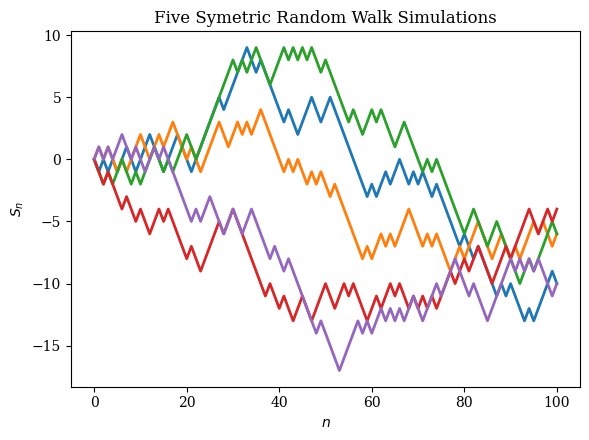
\includegraphics[width=\sOneSize\textwidth]{Chapters/C1/plots/RW_Simulations.png}
    \caption{Three simulations of a symmetric random walk with probability \(p = 0.5\), no drift and no volatility (\(\mu = 0, \sigma = 1\)). Source code: \autoref{ApPy:SymRW}}\label{C1fig:SymRW}
\end{figure}

We let \(S_i \) be the price of an asset on the \(i^{\text{th}}\) day, thus \(S_0\) is the current price of the asset. The drift allows us to model in the expected increase/decrease in price of the asset; scale allows us to model the volatility (the magnitude of movements). There are different methods in which we could employ to calculate our drift and scale parameters, this will typically involve using historical data but can extend to take into account speculation about the underlying asset.

\subsubsection{Drawbacks of a random walk to model asset prices}

We can begin to see how this path may reflect the price an asset which future value is determined by a random event. However, this model comes with several drawbacks: This model only permits the price of the asset to go up and down by a fixed amount, further to this point, the amount is detached from the current value of the asset; we may instead expect that the value change would be proportional to the current value. Lastly, the random walk model also allows asset prices to go negative which typically is considered impossible. However, during April 2020, oil futures became sharply negative for the first time in history~\cite{NegativeOil}. This has lead to people to reconsider the random walk model and see this instead as a positive in specific circumstances. An alternative approach instead applies the random walk model to rate of return instead of asset value, which of course can often be negative.

\subsection{Geometric Brownian motion model}

A better alternative is the (discrete) geometric Brownian model, shown in \autoref{eqn: Geo Brownian Motion}. This model addresses the drawbacks of the simple random walk model. We can see from the left-hand side of the equation, that we now model the percentage increase from the previous time to the current time. This means our price change is not detached from the previous value and the  value can never become negative.

\begin{equation}\label{eqn: Geo Brownian Motion}
    \frac{S_{n+1} - S_n}{S_n} = \delta t\mu + \sqrt{\delta t}\sigma Y_{n}
\end{equation}

Where \(\mu \) is the drift, \(\sigma \) scales the movement and \(Y_i\) are identically and independently distributed (i.d.d.).
\nline{}
On the right-hand side: we introduce a new term, \(\delta t\), this is taken to be a fixed time interval which is comparatively small to the time interval \(t \in [0,T]\); where \(t = T\) is the final time of the model. We let the price of the asset, \(S_i = S(i)\) no longer be measured on the \(i^{\text{th}}\) day, but instead the \(i^{\text{th}}\) number of the time interval \(\delta t\). It is common to calculate \(\delta t\) by considering your entire time range, \(t\in[0,T]\) and splitting this into \(N + 1\) \(\delta t\) increments, where \(N\) is some large number; hence \(S_{N} = S\p{N\delta t} = S\p{T}\). Now, if we were to consider a drift parameter \(\mu \) which represents the expected price increase in one unit of time, it would follow that the increase over our time increment \(\delta t\) would be \(\delta t \mu \). The variance (percentage volatility) of the percentage increase at the final, \(N^{\text{th}}\) step would be \(N\) times the variance at each time interval step, so we would expect this variance to be proportional to \(\delta t\). We let the random component of the percentage increase be proportional to \(\sqrt{\delta t} \); it can be shown that letting \(\sigma \) be proportional to \(\delta t\) or \(\p{\delta t}^{0.25}\) we end up with too little or too much randomness respectively (see \cite{higham2004introduction}). We will again let the values of \( \mu \) and \(\sigma \) be determined in the same manner as previously where we use expert opinion and/or historical data.

\subsubsection{Modified Bernoulli  distributed \(Y_i\)}

We can, as we did previously model the random process in our model, \(Y_i\) as a so-called symmetric random walk; that is:

\begin{equation*}
    Y_i = 
    \begin{cases}
       1& \quad \text{with } P(Y_i = 1) = 0.5; \\
       -1& \quad \text{with } P(Y_i = -1) = 0.5
    \end{cases}
\end{equation*}

\begin{figure}[H]
    \centering
    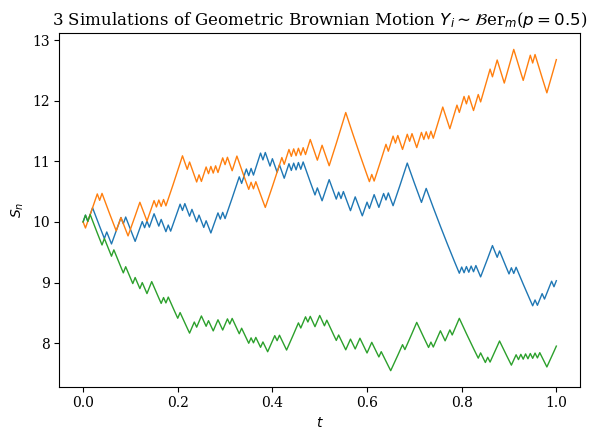
\includegraphics[width=\sOneSize\textwidth]{Chapters/C1/plots/BM_Simulations.png}
    \caption{Three simulations of geometric Brownian motion random walk: with probability \(p = 0.5\), 10\% drift (\(\mu = 0.10\)), volatility 15\% (\(\sigma = 0.15\)) and domain \(t\in[0,1]\) into 201 equal increments. Source code: \autoref{ApPy:GeoRW}}\label{C1fig:GeoSim}
\end{figure}

In \autoref{C1fig:GeoSim} we have simulated geometric Brownian motion over the time range \(t \in [0,1]\). Having \(\mu = 0.10\) means that we expect the path to increase by 10\% for every integer increment in \(t\), thus we would expect \(S_N = (1.1)S_0\) at \( t = N\delta t = T\). Our percentage volatility, \(\sigma = 0.15\) scales our movement at every increment before the drift is applied, this controls the variance or spread of our path. Whilst we have improved significantly from our previous model in \autoref{subsec: RW model}, we still have a restriction in our price change. By having our random process, \(Y_i\) be Bernoulli distributed, we have limited our price change to either increase or decrease by a fixed percentage value.

\subsubsection{Normally distributed \(Y_i\)}

We can then instead distribute \(Y_i\) normally which allows us to add randomness to the amount at which the percentage value changes, instead of just being positive of negative. For instance, we can let \(Y_i \sim \norm\p{0,1}\) then our random process still has equal probability of being positive or negative (since \(\mu = 0\)), but can now vary by random amounts; furthermore it has equal probability to be in some range \([a, b]\) as it is to be in \([-a, -b]\). We set our variance of \(Y_i\) to be one, \(\sigma_Y = 1\), this gives us the standard normal distribution and allows us to alter percentage volatility, \(\sigma \) to account for higher or lower variance; as done previously. \autoref{C1fig:GeoSimNorm} shows three simulations of geometric Brownian motion with standard normal distributed \(Y_i\).
\nline{}
We see how this looks very similar to our previous model, with the exception that it much smoother. Our drift parameter \(\mu \) and percentage volatility \(\sigma \) effect our model in the same way as previously, be it more randomness. You may suspect that in the long run these models will converge to have the same statistical properties. In the next section we will attempt to prove this analytically by letting \(\delta t \rightarrow 0\) and \(N \rightarrow \infty \) and finding a limiting equation of our Brownian motion model.

\begin{figure}[H]
    \centering
    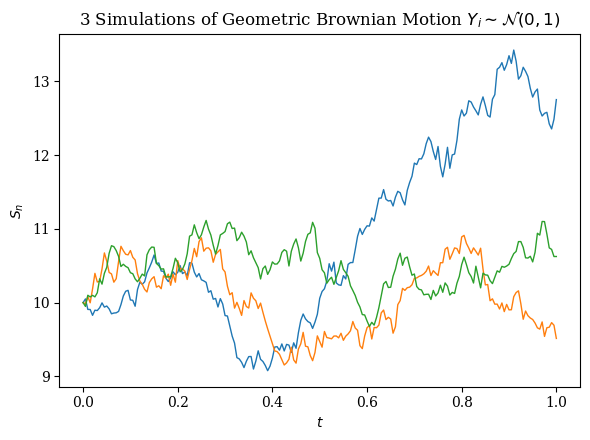
\includegraphics[width=\sOneSize\textwidth]{Chapters/C1/plots/BM_Norm_Simulations.png}
    \caption{Three simulations of geometric Brownian motion with 10\% drift (\(\mu = 0.10\)), volatility 15\% (\(\sigma = 0.15\)) and domain \(t\in[0,1]\) into 201 equal increments. Source code: \autoref{ApPy:GeoNorm}}\label{C1fig:GeoSimNorm}
\end{figure}

\subsubsection{Comparing normal and modified Bernoulli distributed \(Y_i\)}

Let us rewrite our geometric Brownian motion model as follows:

\begin{equation}\label{eqn: GeoBrown Model}
    S_{n+1} = S_n + S_n\delta t\mu + S_n\sqrt[]{\delta t}\sigma Y_{n}
\end{equation}

Now, again consider a time interval \(t\in[0,T] \) where \(T = N\delta t\). We know \(S(0) = S_0 \) and \autoref{eqn: GeoBrown Model} gives us an expression for \(S(\delta t)=S_1,\;\dots \;,S(T) = S_N\). We now let \(\delta t \rightarrow 0 \implies N \rightarrow \infty \) and find a limiting equation for \( S_n \). \autoref{eqn: GeoBrown Model} tells us at each \(\delta t\) interval we multiply the asset price by \(1+\mu\delta t+\sqrt{\delta t}\sigma Y_n\). Thus, we can write \(S(T) \) as:

\begin{equation*}
    S(T) = S_0\prod_{n=0}^{N-1}\p{1+\mu\delta t+\sqrt{\delta t}\sigma Y_n}
\end{equation*}

Now, diving by \(S_0 \) and taking the log:

\begin{equation}\label{}
    \log\p{\frac{S(T)}{S(0)}} = \sum_{n=0}^{N-1}\log\p{1+\mu\delta t+\sqrt{\delta t}\sigma Y_n}
\end{equation}

We are interested in the limit \(\delta t \rightarrow 0\), so we would like to exploit the Taylor expansion \(\log(1 + x) \approx x - \frac{x^2}{2} + \BigO{x^3} \), for small \(x\). It is worth noting the quantity \(Y_n\) in \autoref{eqn: GeoBrown Model} is a RV, not a number. It can however be shown that if \(\E{Y_n^2}\) is finite, then we can treat \(Y_i\) as a number for our approximation~\cite{higham2004introduction}. Continuing such that the log expansion remains valid, we obtain:

\begin{align}\label{eqn: GeoBrownExpansion}
    \log\p{\frac{S(T)}{S(0)}} \approx \sum_{n=0}^{N-1} \p{\mu\delta t + \sigma\sqrt{\delta t}Y_n - \frac{1}{2}\sigma^2\delta tY_n^2} + \BigO{\delta t^\frac{3}{2}}
\end{align}

Where terms of \(\delta t^\frac{3}{2}\) or higher have been omitted.
\nline{}
Now, if we consider the Expectation and Variance of \(\p{\mu\delta t + \sigma\sqrt{\delta t}Y_n - \frac{1}{2}\sigma^2\delta tY_n^2}\):

\begin{align*}
    \begin{split}
        \E{\mu\delta t + \sigma\sqrt{\delta t}Y_n - \frac{1}{2}\sigma^2\delta tY_n^2} &=  \mu\delta t + \sigma\sqrt{\delta t}\E{Y_n} - \frac{1}{2}\sigma^2\delta t\E{Y_n^2} \\
        &= \mu\delta t + \sigma\sqrt{\delta t}\E{Y_n} - \frac{1}{2}\sigma^2\delta t\p{\var{Y_n} + \E{Y_n}^2}
    \end{split}
    \\
    \begin{split}
        \var{\mu\delta t + \sigma\sqrt{\delta t}Y_n - \frac{1}{2}\sigma^2\delta tY_n^2} &= \sigma^2\delta t\var{Y_n} - \frac{1}{4}\sigma^4\delta t^2\var{Y_n^2} \\
        &= \sigma^2\delta t\var{Y_n} + \BigO{\delta t^\frac{3}{2}}
    \end{split}
\end{align*}

We can see that both our equations above depend on the expectation and variance of \(Y_n\). For both our modified Bernoulli and normally distributed \(Y_i\) we can show that \(\E{Y_i} = 0\) and \(\var{Y_i} = 1\). Thus, for both of our Brownian motion models we can rewrite our above equations as:
\begin{align*}
    \begin{split}
        \E{\mu\delta t + \sigma\sqrt{\delta t}Y_n - \frac{1}{2}\sigma^2\delta tY_n^2} &= \mu\delta t - \frac{1}{2}\sigma^2\delta t
    \end{split}
    \\
    \begin{split}
        \var{\mu\delta t + \sigma\sqrt{\delta t}Y_n - \frac{1}{2}\sigma^2\delta tY_n^2} &= \sigma^2\delta t + \BigO{\delta t^\frac{3}{2}}
    \end{split}
\end{align*}

Since our realizations of \(Y_i\) are i.i.d.~and our RHS contains no RVs, we can use the following:

\begin{align*}
    \E{\sum_{i=0}^N f(x)} = N\cdot\E{f(x)} && \var{\sum_{i=0}^N f(x)} = N\cdot\E{f(x)}
\end{align*}

Now using the Central Limit Theorem we can approximate \autoref{eqn: GeoBrownExpansion} as a normally distributed variable with mean \(N\p{\mu\delta t - \frac{1}{2}\sigma^2\delta t} = T\p{\mu - \frac{1}{2}\sigma^2}\) and variance \(N\p{\sigma^2\delta t + \BigO{\delta t^\frac{3}{2}}} = T\sigma^2\), since \(N\delta t = T\). So we have the following approximation for large \(N\) and relatively small \(\delta t\) over the range \(t\in[0,T]\).

\begin{equation}\label{eqn: Asset Log Dist}
    \log\p{\frac{S(T)}{S(0)}} \sim \norm\p{\mu - \frac{1}{2}\sigma^2,\; T\sigma^2}
\end{equation}

We may be surprised to see an extra term in the mean of our normal distribution in \autoref{eqn: Asset Log Dist}. One may expect our mean to simply be the time period multiplied by expected rate of return (drift), but this extra term arrives from the random noise in our Brownian model. This occurs because the path is not smooth, although continuous; the path is not everywhere differentiable. This is why it was required that we went to the quadratic term in our Taylor expansion of \(\log\p{1+x}\) to get the correct linear approximation of \(\log\p{S(T)/S(0)}\).
\nline{}
Our limiting continuous time expression for our asset model, using either a modified Bernoulli or normally distributed \(Y_i\) (or any distribution centred zero, variance equal to 1 and finite second moment) becomes:

\begin{equation}\label{eqn:c1:S(T)}
    S(T) = S_0\exp^{\p{\mu-\frac{1}{2}}T+\sigma\sqrt{T}Z},\quad\text{Where \(Z\sim\norm\p{0,1}. \)}
\end{equation}

It is worth noting that there was nothing in our derivation that required us to use \(t = 0 \text{ and } t = T\), we could in fact use any two values \(S_i, S_j\;:\; i < j\in [0,N]\). With \(0 \leq i < j \leq N\), we have:

\begin{equation}\label{eqn:c1: i,j log distribution}
    \log\p{\frac{S(j\delta t)}{S(i\delta t)}} \sim \norm\p{\p{\mu - \frac{1}{2}\sigma^2}\p{j-i}\delta t,\;\p{\sigma^2\p{j-i}\delta t}}
\end{equation}

Since our \(Y_i\) are i.i.d.~across non-overlapping intervals, the normal RVs that describe these changes will be independent. Thus, \(\forall i,j,k \in [0,N]\; : \; i < j < k\), we have:

\begin{equation*}
    \log\p{\frac{S(k\delta t)}{S(j\delta t)}} \sim \norm\p{\p{\mu - \frac{1}{2}\sigma^2}\p{k-j}\delta t,\;\p{\sigma^2\p{k-j}\delta t}}
\end{equation*}

Which is independent of \(\log\p{\frac{S(j\delta t)}{S(i\delta t)}}\).
\nline{}
Thus, we can describe our asset price modelled by our geometric Brownian motion over any sequence of time points using the following equation:

\begin{equation}\label{eqn:c1:geobrown model}
    S_{n+1} = S_n\exp^{\p{\mu-\frac{1}{2}\sigma^2}\p{\delta t} + \sigma\sqrt{\delta t}Z_i}, \quad \text{With i.i.d.~} Z_i \sim \norm\p{0,1}.
\end{equation}

So as it turns out, it does not matter how we decide to distribute \(Y_i\) so long as the \(\E{Y_i} = 0, \var{Y_i} = 1 \text{ and } \E{Y_i^2}\) is finite; we end up with a statistically equivalent model, for large \(N\) and a small \(\delta t\) relative to the time interval \(t\in[0,T]\). 
\nline{}
The above is an important derivation to know when deciding how to correctly choose parameters in the binomial method of pricing options, as done in \autoref{subsubsec: Binomial method}.

\section{Pricing standard options}

Since the holder of the contract is not obliged to exercise the contract at the expiry time, they do not hold any liability in the absence of a price to purchase the option. The problem then becomes, what is the correct price to charge the holder of the option to balance this inequality of liability.

\subsection{Black-Scholes Model}

\begin{equation}\label{eqn:BS}
    \frac{\partial \pof}{\partial t} + \frac{1}{2}\sigma^2S^2\frac{\partial^2\pof}{\partial S^2} + rS\frac{\partial \pof}{\partial S} - r\pof = 0
\end{equation}

The Black Scholes Equation is a partial differential equation developed by two economists, Fisher Black and Myron Scholes. This equation shows the value of an option as a function of time and underlying asset value. Thus, solving this equation with an appropriately chosen boundary conditions you can in some cases find an analytical solution to price an option. Most famously, Black and Scholes showed that with a change of variables transformation, it was possible to transform the Black-Scholes equation for a European put or call option into the commonly solved heat equation. Upon solving and transforming the variables back, they had provided an analytical solution for a European put and call option.

\subsection{Deriving the Black-Scholes equation}

The following derivation is taken from an unpublished report~\cite{Yr2Project}, which follows works from Hull~\cite{hull2012options} which is in turn is based on the classic argument given in the original Black-Scholes paper~\cite{black1973pricing}. To derive the Black-Scholes Equation we must first make three assumptions about the price of an option.

\begin{enumerate}
    \item The stock price follows a stochastic process, meaning that we can not use historical price to predict its future movement.
    \item The option pays no dividends to the owner.
    \item Risk-free rate, \(r\) and percentage volatility, \(\sigma \) are known and constant.
\end{enumerate}

We again assume that the price of an asset follows a geometric Brownian motion. However, we instead opt for the continuous form, that is:

\begin{equation}\label{Brownian}
    \frac{dS}{S} = \mu dt + \sigma dW
\end{equation}

Where \(W\) is a stochastic variable (Brownian motion). Note that \(W \), and consequently its infinitesimal increment \(dW \), represents the only source of uncertainty.

The payoff of an option \(\pof(S,t) \) at the exercise date, \(t = T\) is known. To find the value of the option at an earlier time, we need to know how \(\pof \) changes as a function of \(S \) and \(t \).

As we have assumed \(\pof(S,t) \) is a stochastic process and also dependent on time we can find the differential of \(\pof \) using Itō's lemma. 

By Itō's lemma for two variables we have:

\begin{equation}\label{Ito}
    d\pof = \bigg( \mu S \frac{\partial \pof}{\partial S} + \frac{\partial \pof}{t} + \frac{1}{2}\sigma^2 S^2 \frac{\partial^2 \pof}{\partial S^2}\bigg)dt + \sigma S \frac{\partial \pof}{\partial S}dW
\end{equation}

Now, consider a specific portfolio, the delta-hedge portfolio, consisting of the negative value of the option and \(\frac{\partial \pof}{\partial S} \) shares at time \(t \). The value of the portfolio is then:

\begin{equation*}
    \Pi = -\pof + \frac{\partial \pof}{\partial S}S
\end{equation*}

Over a given time period, the total profit or loss from changes in the values of the holdings (the option and shares) is

\begin{equation}\label{deltahedge}
    \Delta \Pi = -\Delta \pof + \frac{\partial \pof}{\partial S}\Delta S
\end{equation}

Now discretizing equations~\eqref{Brownian} and~\eqref{Ito}:

\begin{align*}
    \Delta S &= \mu S \Delta t + \sigma S \Delta W , & \Delta \pof = \bigg(\mu S \frac{\partial \pof}{\partial S} + \frac{\partial \pof}{\partial t} + \frac{1}{2}\sigma^2S^2\frac{\partial^2\pof}{\partial S^2}\bigg)\Delta t + \sigma S \frac{\partial \pof}{\partial S} \Delta W
\end{align*}

and substituting these into \autoref{deltahedge}, we obtain

\begin{equation}\label{LHS}
    \Delta \Pi = \bigg(-\frac{\partial \pof}{\partial t} - \frac{1}{2}\sigma^2S^2\frac{\partial^2\pof}{\partial S^2}\bigg)\Delta t
\end{equation}

Note that \(\Delta W \) term has vanished. Thus, uncertainty has been eliminated, and the portfolio is effectively risk-less. The rate of return on this portfolio must be equal to the rate of return on any other risk-less instrument; otherwise, there would be opportunities for arbitrage. Now given the risk-free rate of return is \(r \), we must have over the same given time period:

\begin{equation}\label{RHS}
    r\Pi \Delta t = \Delta \Pi
\end{equation}

Now equating our two formulas for \(\Delta \Pi \), equations~\eqref{LHS} and~\eqref{RHS}

\begin{equation*}
    \bigg(-\frac{\partial \pof}{\partial t} - \frac{1}{2}\sigma^2S^2\frac{\partial^2\pof}{\partial S^2}\bigg)\Delta t = r\bigg(-\pof+S\frac{\partial \pof}{\partial S}\bigg)\Delta t
\end{equation*}

Simplifying, we arrive at the celebrated Black-Scholes equation:

\begin{equation*}
    \frac{\partial \pof}{\partial t} + \frac{1}{2}\sigma^2S^2\frac{\partial^2\pof}{\partial S^2} + rS\frac{\partial \pof}{\partial S} - r\pof = 0
\end{equation*}

With the assumptions of the Black-Scholes model, this second order partial differential equation holds for any type of option as long as its payoff function depends only on the underlying asset value at the expiry date and its price function \(\pof \) is twice differentiable with respect to \(S \) and once with respect to \(t \).

\subsection{Risk-neutrality assumption}

Before the publication of the Black-Scholes model, it was thought that the value of an option should be equal to it's expected payoff, for a European styled option; that is:

\begin{equation*}
    W\p{T,S(T)} = \E{e^{-rT}\poff{S(T)}} 
\end{equation*}

Where \(T\) is the option's expiry date, \(r\) the risk-free interest rate, \(\pof(t)\) the payoff function of the option and \(S(T)\) is the underlying asset value at time \(t\). Remembering back to our asset model, we know \(S(T) \) is a random variable from \autoref{eqn:c1:S(T)}. We may consider our option value at any \(t \in [0,T]\) as being:

\begin{equation}\label{eqn:c1:disfpayoff}
    W\p{t,S(T)} = e^{-r(T-t)}\E{\poff{S(T)\;|\;S(t)}} 
\end{equation}

Which may be written explicitly using our asset model and properties of RVs. We shall leave in this implicit form for brevity. This may seem like a reasonable approach to value an option. However, this equation has made no attempt to mitigate risk through the use of hedging; nor has it been derived with the no arbitrage principle we established in \autoref{subsubsec: No Arb} in mind. More importantly our equation depends on our drift parameter \(\mu \).
\nline{}
The no-arbitrage principle tells us that there can only be one fair value for an option, and that is the one quoted in the market. If the value was higher or lower an opportunity for arbitrage would occur giving investors risk-free profit. This restricts the value of the option to the Black-Scholes level, it follows that since our discounted expected payoff method depends on \(\mu \); that it cannot be used to get a fair value.
\nline{}
However, as it turns out if we assume what is called risk-neutrality assumption; that is we let our drift parameter be equal to our risk-free interest, i.e. \(\mu = r\). Then we arrive at the remarkable conclusion that our expected discounted payoff, \autoref{eqn:c1:disfpayoff} satisfies our Black-Scholes PDE, \autoref{eqn:BS}.
\nline{}
We summarize the risk-neutrality assumption as follows: regardless of the parameters \(\sigma\) and \(\mu\) we believe to be correct in our asset model \autoref{eqn:c1:geobrown model}. If we suppose that our drift \(\mu\) is instead equal to our risk-free interest rate \(r\) than by using the discounted expected payoff we can obtain the Black-Scholes option value. 
\nline{}
In the risk-neutral world we have that the expected price of an asset is just the same as investing the value of the initial asset risk-free, i.e. \(\E{S(t)} = S_0\exp\p{rt}\). This kind of process, one in which the expected future value is equal to the initial value is called a martingale process. Through martingale theory one can use the risk-neutrality assumption to price options consistent with the no-arbitrage principle~\cite{kritzman2000puzzles}. This proves to be a powerful tool when valuing options using numerical methods, we will see this in our next model \autoref{subsubsec: Binomial method} and \autoref{subsec: Asian Models}.

\subsection{Binomial method}\label{subsubsec: Binomial method}

The binomial option pricing model (BOPM) provides a generalized discrete numerical method for valuing options. The model uses a binomial tree where at each discrete time-step the underlying asset goes up or down by a fixed (percentage) value. It was first proposed by William Sharpe in 1978~\cite{sharpe1978investments}, but formalized by Cox, Ross and Rubinstein in 1979~\cite{COX1979229}. Since then, many developments and improvements have been made; here we will follow closely to D.~Higham work~\cite{higham2004introduction}.

\subsubsection{Binomial model over a single time-step}

We will first consider a one-step binomial model. In this model we have an underlying asset with current (initial) price, \(S_0\). We propose in one time-step from \(t = 0\) to \(t = 1 = T\) that the price will either change to \(S_T = uS_0\) or \(S_T = dS_0\) where \(d < u\); with probabilities \(p\) and \(\p{1-p}\) respectively. We write this as follows:

\begin{align*}
    S_T 
    =
    \begin{cases}
        uS_0 = \inc{S}{1}{1} \quad \text{with }P\p{S_T=\inc{S}{1}{1}} = p \\
        dS_0 = \inc{S}{1}{0} \quad \text{with }P\p{S_T=\inc{S}{1}{0}} = \p{1-p}
    \end{cases}
\end{align*}
The notation \(\inc{S}{i}{j}\) simply represents the value of the underlying asset at the \(i^\text{th}\) time-step with \(j\) up steps, note that the number of down steps is simply \(i-j\).
\nline{}
We may also construct a lattice that describe the potential paths of the underlying asset value, this becomes useful when we increase the number of steps. Similarly, we construct a lattice which describes the value of the option given the corresponding value of the underlying asset. These are both shown in \autoref{tree:c1:onestep both}

\begin{figure}[H]
    \centering
    \begin{subfigure}[b]{0.49\textwidth}
        \centering
        \begin{tikzpicture}[>=stealth,sloped]
            \matrix (tree) [%
            matrix of nodes,
            minimum size=0.25cm,
            column sep=3.5cm,
            row sep=0.5cm,
            ]
            {
                        & \(uS_0\) \\
                \(S_0\) &          \\
                        & \(dS_0\) \\
            };
            \draw[->] (tree-2-1) -- (tree-1-2) node [midway,above] {\(p\)};
            \draw[->] (tree-2-1) -- (tree-3-2) node [midway,below] {\(\p{1-p}\)};
        \end{tikzpicture}
        \subcaption{Possible asset values for \(t\in[0,T]\)}\label{tree:c1:1step asset}
    \end{subfigure}
    \begin{subfigure}[b]{0.49\textwidth}
        \centering
        \begin{tikzpicture}[>=stealth,sloped]
            \matrix (tree) [%
              matrix of nodes,
              minimum size=0.25cm,
              column sep=3.5cm,
              row sep=0.5cm,
            ]
            {
                                    & \(\inc{\pof}{1}{1}\) \\
                \(\inc{\pof}{0}{0}\)   &          \\
                                    & \(\inc{\pof}{1}{0}\) \\
            };
            \draw[->] (tree-2-1) -- (tree-1-2) node [midway,above] {\(p\)};
            \draw[->] (tree-2-1) -- (tree-3-2) node [midway,below] {\(\p{1-p}\)};
        \end{tikzpicture}
        \subcaption{Possible option values for \(t\in[0,T]\)}\label{tree:c1:1step option}
    \end{subfigure}
\caption{Two binomial trees which represent the evolution of the underlying asset value, and the value of the option from \(t = 0\) to \(t = T\).}\label{tree:c1:onestep both}
\end{figure}

We know how to calculate the options value at \(t=T\), this simply requires inputting the corresponding \(S_T \) values into the options payoff function; i.e.~for a standard European put option with strike price, \(E \) expiring at \(t = T\) the payoff function is such:

\begin{equation*}
    \poff{S_T} = \max\p{E-S_T,\;0}
\end{equation*}

Substituting our potential \(S_T\) tells us the possible values of the option at \(t=T\), let \(dS_0 < E < uS_0\):

\begin{align*}
    X(S_T) 
    =
    \begin{cases}
        0 &\quad \text{if }S_T=\inc{S}{1}{1} \\
        E-dS_0 &\quad \text{if }S_T=\inc{S}{1}{0}
    \end{cases}
\end{align*}

We must now determine the value of \(\inc{\pof}{0}{0}\), a natural method may be to calculate the discounted expected payoff of the option; that is the amount you would need to invest risk-free to guarantee \(\E{\pof(S_T)}\) at \(t=T\); this depends on the probability \(p\). However, as mentioned previously, doing so leads to an answer which is not consistent with our No-Arbitrage assumption. To price the option consistent with the No-Arbitrage assumption we must calculate the risk-neutral probability, \(p_*\) this is the probability in which our discounted expected payoff value is equal to the initial option value; becoming a martingale process. It can be shown that the same probability \(p_*\), satisfies expected discounted asset value being equal to the initial asset value~\cite{kritzman2000puzzles}, i.e.:

\begin{equation*}
    \Ep{p_*}{e^{-r\delta t}S_{\delta t}} = e^{-r\delta t}\s{p_*\inc{S}{1}{1} + \p{1-p_*}\inc{S}{1}{0}} = S_0
\end{equation*}

Here \(\delta t = \p{T-0} = T\) which is the change in time in one step, it is also worth noting that this value holds across all steps. It follows that we can calculate the risk-neutral probability, \(p_*\) using the following:

\begin{equation}\label{eqn: Risk Neutral Prob}
    p_* = \frac{S_0e^{r\delta t} - uS_0}{uS_0 - dS_0} = \frac{e^{r\delta t} - u}{u - d}
\end{equation}

We can then use \(p_*\) to find the value of the option at time \(t = 0\).

\begin{equation*}
     \Ep{p_*}{e^{-rT}\pof_{\delta t}} = e^{-rT}\s{p_*\inc{\pof}{1}{1} + \p{1-p_*}\inc{\pof}{1}{0}} = \inc{\pof}{0}{0}
\end{equation*}

\subsubsection{Extending to multiple steps}

Now extending our method over multiple time-steps, let expiry time \(T = 2\) and \(\delta t = 1\). We construct the following lattice

\begin{figure}[H]
    \centering
    \begin{tikzpicture}[>=stealth,sloped]
        \matrix (tree) [%
          matrix of nodes,
          minimum size=0.25cm,
          column sep=3.5cm,
          row sep=0.5cm,
        ]
        {
                                &                       & \(\inc{\pof}{2}{2}\) \\
                                & \(\inc{\pof}{1}{1}\)     &                   \\
            \(\inc{\pof}{0}{0}\)   &                       & \(\inc{\pof}{2}{1}\) \\
                                & \(\inc{\pof}{1}{0}\)     &                   \\
                                &                       & \(\inc{\pof}{2}{0}\) \\
                    \(t=0\) & \(t=1\) & \(t=2\) \\
        };
        \draw[->] (tree-3-1) -- (tree-2-2) node [midway,above] {};
        \draw[->] (tree-3-1) -- (tree-4-2) node [midway,below] {};
        \draw[->] (tree-2-2) -- (tree-1-3) node [midway,above] {};
        \draw[->] (tree-2-2) -- (tree-3-3) node [midway,below] {};
        \draw[->] (tree-4-2) -- (tree-3-3) node [midway,above] {};
        \draw[->] (tree-4-2) -- (tree-5-3) node [midway,below] {};
    \end{tikzpicture}
    \caption{A binomial tree representing the possible option values from \(t = 0\) to \(t = 2\) with \(\delta t = 1\)}\label{}
\end{figure}

We can see at both nodes when time, \(t = 1\), we essentially have two one-step binomial models. If we apply the one-step method to each, we can then use our calculated values to find our current option value.
\nline{}
It follows that we can do this for any number of steps, let expiry time \(T = N\). Then we begin by calculating the payoff for each node in the final column, i.e. \(\inc{\pof}{N}{k} = \pof(u^k d^{N-k}S_0)\) at time \(t=N\). Using these values we can then calculate the nodes at the previous time step, i.e.~time \(t = m = N-1\):

\begin{equation}\label{eqn:c1:binomial method eqn}
    \inc{\pof}{m}{k} = e^{-r\delta t}\p{p_*\inc{\pof}{m+1}{k+1} + \p{1-p_*}\inc{\pof}{m+1}{k}}
\end{equation}

This can then be repeated for the next previous step, \(t = m = N-2\), and so forth. This is repeated until \(m = 0\), at which point you will have calculated the initial option value.

\subsubsection{Determining Parameters}

Let us assume that you have determined appropriate values for drift, \(\mu \) and percentage volatility, \(\sigma \) through use of historical data or expert speculation. We may ask how can these values be used to determine the value of our up step, \( u\) and or down step \(d \). 
\nline{}
Let us describe out underlying asset path using a Bernoulli distributed RV, \(\beta_i\). Let \(\beta_i = 1\) with when our asset steps up over a single time step from\((i-1)\delta t\) to \(i\delta t\), and \(\beta_i = 0\) when we step down. Hence, we can write out path as follows:

\begin{equation*}
    S(n\delta t) = S_0u^{\sum_{i=1}^n\beta_i}d^{n-\sum_{i=1}^n\beta_i}
\end{equation*}

We rearrange this to the following:

\begin{equation}
    \frac{S(n\delta t)}{S_0} = d^n\p{\frac{u}{d}}^{\sum_{i=1}^n\beta_i}
\end{equation}

Then taking logs:

\begin{equation*}
    \log\p{\frac{S(n\delta t)}{S_0}} = n\log\p{d} + \sum_{i=1}^n\beta_i\log\p{\frac{u}{d}}
\end{equation*}

Now continuing as we did in \autoref{eqn: GeoBrownExpansion}, whereby we calculated the expectation and variance of our log expression, using \(\E{\beta_i} = p,\; \var{\beta_i} = p\p{1-p}\) since \(\beta_i\) is a standard Bernoulli RV~:

\begin{align*}
    \begin{split}
        \E{n\log\p{d} + \sum_{i=1}^n\beta_i\log\p{\frac{u}{d}}} &= n\log\p{d} + \log\p{\frac{u}{d}}\sum_{i=1}^n\E{\beta_i} \\
    &= n\log\p{d} + np\log\p{\frac{u}{d}} \\
    &= n\s{\log\p{d} + p\p{\logp{u} - \logp{d}}} \\
    &= n\s{p\logp{u} + \p{1-p}\logp{d}}
    \end{split}
    \\
    \begin{split}
        \var{n\log\p{d} + \sum_{i=1}^n\beta_i\log\p{\frac{u}{d}}} &= \logp{\frac{u}{d}}^2 \sum_{i=1}^n\var{\beta_i} \\
        &= n\s{p\p{1-p}\logp{\frac{u}{d}}^2}
    \end{split}
\end{align*}

Now, if we apply the Central Limit Theorem for large \(n\) and assume our underlying asset should match our Brownian motion equations. Then \autoref{eqn:c1: i,j log distribution} tells us the mean of \({\logp{S(n\delta t)}/{S_0}} \) must equal \(\p{\mu - \frac{1}{2}\sigma^2}n\delta t\) and the variance be \(\sigma^2n\delta t\). Hence, we get the following equations:

\begin{align}\label{eqn:c1:paramater match exp and var}
    \begin{split}
        \s{p\logp{u} + \p{1-p}\logp{d}} &= \p{\mu - \frac{1}{2}\sigma^2}\delta t
    \end{split}
    &&
    \begin{split}
        \s{p\p{1-p}\logp{\frac{u}{d}}^2} &= \sigma^2\delta t \\
        \logp{u} - \logp{d} &= \sigma\sqrt{\frac{\delta t}{p\p{1-p}}}
    \end{split}
\end{align}

Now, since we determine \(\mu, \sigma \) and \(\delta t = {T}/{N} \); it stands that we have three unknowns, \(u, d, p\) for two equations. It follows that we must then fix one of our unknowns, or determine a third equation. A popular choice is to fix \(d = {1}/{u}\) and consider that when we price our option we do not use parameter \(p\), we do however use \(u \) and \(d \) in the calculation. The definition of our drift, \(\mu \) tells us that it should be closely related to \(p\). Thus, we can conclude that \(u \) and \(d \) should not dependent on \(\mu\), but instead solely on the percentage volatility \(\sigma\). Whilst many solutions can exist we will use the following:

\begin{align*}
    u = e^{\sigma\sqrt{\delta t}}
    &&
    d = e^{-\sigma\sqrt{\delta t}}
\end{align*}

Which leads to the following expression for \(p \):

\begin{equation*}
    p = \frac{1}{2} + \frac{1}{2\sigma}\p{\mu -\frac{1}{2}\sigma^2}\sqrt{\delta t}
\end{equation*}

Substituting these values into \autoref{eqn:c1:paramater match exp and var} confirms their accuracy to \(\BigO{\delta t^\frac{3}{2}}\) as required. It is worth noting this is not the only way to determine \(u, d, p\) from \(\mu, \sigma, \delta t\). Some notable examples are: \(u = \exp\p{\sigma\sqrt{\delta t}+\p{r-{1}/{2}}\delta t}, d = {1}/{u}\)~\cite{higham2004introduction} and \(u = \exp\p{\delta t}\p{1+\sqrt{\exp\p{\sigma^2\delta t}-1}}, \; d = \exp\p{\delta t}\p{1-\sqrt{\exp\p{\sigma^2\delta t}-1}}\)~\cite{wilmott1995mathematics}.

\subsubsection{Overview of the BOPM}

The BOMP is a very robust model allowing you to easily implement different payoff function into the algorithm, since you calculate values one node at a time. This makes it easy to implement break conditions, such as a so-called All or Nothing option; an option format where if a price of an underlying asset drops below an exercise price at any time \(t \leq T\), it is worth nothing. It is for this reason the binomial method is a good choice to price American options since they can be exercised at any time \(t \leq T\).
\nline{}
One of the biggest benefits is the relative simplicity of the model it is quite straight forward to programme an algorithm that implements the method without involving any complicated mathematics. However, a drawback to the method is that for options in which the number of computations grow exponentially relative to the number of time-steps.~i.e.~For Asian options, we need to calculate the average off all different possible paths so as \(N\) becomes large, this becomes computationally unviable. Hence, it is required that we modify the method; we will explore this in \autoref{subsec: Asian Models}.

\section{Pricing Asian options}\label{subsec: Asian Models}

In this section we will explore several methods which can be used to price Asian options. Whilst an analytical solution exists for Asian options which use a geometric average~\cite{zhang1997exotic}; it not the case when we use the more popular arithmetic average. Asian options which use an arithmetic average must instead be solved using numerical approaches.

\subsection{Pricing Asian options using BOPM}

Let us again consider an asset with an initial value \(S_0 = 10\), with a probability \(p = 0.5\) of going up to \(uS_0\) or down to \(dS_0\) at every time-step \(\delta t = 0.1\) with \(u=1.1,\;d=1/u\). We can again show this in a binomial tree, however, we will also show the potential path dependent arithmetic averages that can be reached at each node. This can be seen in \autoref{tree:c1:asian averages}.
\nline{}
Suppose \(3\delta t = T\), then we are able to calculate the value of the option at \(t=T\) for each possible path. We introduce the notation \(\inct{S}{i}{j}{k}\) as being the asset (or option) value at the \(i\) time-step, with \(j\) up steps and \(k^{th}\) possible value, where \(k_1 > k_2 > \dots \). Thus, from figure \autoref{tree:c1:asian averages} \(\inct{S}{3}{2}{2} = 10.50\).

\begin{figure}[H]
    \centering
    \begin{tikzpicture}[>=stealth,sloped]
        \matrix (tree) [%
            matrix of nodes,
            minimum size=1cm,
            column sep=1.0cm,
            row sep=0.25cm,
        ]
        {
                                        &                                   &                                       & \nd[11.60]{\incm{S}{3}{3}\(=13.31\)}              \\
                                        &                                   & \nd[11.03]{\incm{S}{2}{2}\(=12\).1}       &                                               \\
                                        & \nd[10.50]{\incm{S}{1}{1}\(=11\)}     &                                       & \ndt[11.02][10.50][10.02]{\incm{S}{3}{2}\(=11\)}  \\
            \nd[10]{\incm{S}{0}{0}\(=10\)}  &                                   & \nd[10.33][9.70]{\incm{S}{2}{1}\(=10\)}   &                                               \\
                                        & \nd[9.54]{\incm{S}{1}{0}\(=9.09\)}    &                                       & \ndt[10.02][9.55][9.11]{\incm{S}{3}{1}\(=9.09\)}  \\
                                        &                                   & \nd[9.11]{\incm{S}{2}{0}\(=8.26\)}        &                                               \\
                                        &                                   &                                       & \nd[8.72]{\incm{S}{3}{0}\(=7.51\)}                \\
                                        \(t=0\delta t\) & \(t=1\delta t\) &\(t=2\delta t\) &\(t=3\delta t\) \\
        };
        \draw[->] (tree-4-1) -- (tree-3-2) node [midway,above] {};
        \draw[->] (tree-4-1) -- (tree-5-2) node [midway,below] {};
        \draw[->] (tree-3-2) -- (tree-2-3) node [midway,above] {};
        \draw[->] (tree-3-2) -- (tree-4-3) node [midway,below] {};
        \draw[->] (tree-5-2) -- (tree-4-3) node [midway,above] {};
        \draw[->] (tree-5-2) -- (tree-6-3) node [midway,below] {};
        \draw[->] (tree-2-3) -- (tree-1-4) node [midway,below] {};
        \draw[->] (tree-2-3) -- (tree-3-4) node [midway,below] {};
        \draw[->] (tree-4-3) -- (tree-3-4) node [midway,below] {};
        \draw[->] (tree-4-3) -- (tree-5-4) node [midway,below] {};
        \draw[->] (tree-6-3) -- (tree-5-4) node [midway,below] {};
        \draw[->] (tree-6-3) -- (tree-7-4) node [midway,below] {};
    \end{tikzpicture}
    \caption{A binomial-tree representing the potential assets values with the corresponding path averages below. \(S_0 = 10,\;u=1.1,\;d=1/u,\;\delta t = 0.1\)}\label{tree:c1:asian averages}
\end{figure}

Let our option be a fixed-strike price Asian call option, in which the arithmetic average taken every \(\delta t = 0.1\) is used as the spot price with strike price \(E = 10\). Then using \autoref{tree:c1:asian averages} we can proceed to calculate our option value at \(t = T\), we will calculate for both \(\inct{\pof}{3}{3}{k}\) and \(\inct{\pof}{3}{2}{k}\)

\begin{align*}
    \begin{split}
        \inct{\pof}{3}{3}{1} &= \max\p{13.31-10,0} = 3.31
    \end{split}
    &&
    \begin{split}
        \inct{\pof}{3}{2}{1} &= 1.02 \\
        \inct{\pof}{3}{2}{2} &= 0.50 \\
        \inct{\pof}{3}{2}{3} &= 0.02 \\
    \end{split}
\end{align*}

Now, as it stands we are able to use \autoref{eqn:c1:binomial method eqn} to work backwards and price \(\inct{\pof}{2}{2}{1}\). We just need to make a slight adjustment to the formula and select \(k_u\) such that the \(k_u^{th}\) option value is the value in which we arrive after an up step from \(\inct{\pof}{i}{j}{k}\); similarly \(k_d\) to arrive at the correct down step.

\begin{equation}\label{eqn:asian binomial eqn}
    \inct{\pof}{i}{j}{k} = e^{-r\delta t}\p{p_*\inct{\pof}{i+1}{j+1}{k_u} + \p{1-p_*}\inct{\pof}{i+1}{j}{k_d}}
\end{equation}

This gives us the following equation for \(\inct{\pof}{2}{2}{1}\)

\begin{align*}
    \inct{\pof}{2}{2}{1} &= e^{-r\delta t}\p{p_*\inct{\pof}{3}{3}{1} + \p{1-p_*}\inct{\pof}{3}{2}{1}} \\
    &= e^{-r\delta t}\p{p_*3.31 + \p{1-p_*}1.02}
\end{align*}

As we did with the standard BOPM we can repeat this process for all nodes and their respective path dependent averages, working backwards till we reach \(\inct{\pof}{0}{0}{0}\), giving us the present value of the option.

\subsubsection{Difficulties with BOPM}

As mentioned previously, the standard BOPM comes into problems when applied to Asian type options. Let us again consider a binomial tree to describe our asset value, then at each time-step (\(\delta t\)) our number of possible asset values increases by \(\delta t + 1\). Thus, for \(N \) steps we have \(\sum_{i=0}^N i + 1 = \frac{1}{2}\p{N+1}\p{N+2} \sim \BigO{N^2}\) different nodes. As seen in the binomial method, we have to calculate the value of the option at each corresponding node. For a standard option this is just one calculation per node, giving us \(\approx N^2\) calculations. However, the value of an Asian option at each node depends on the path taken to reach it. Thus, to calculate the value at each node we must calculate for every potential path that can be taken; as for every deviation in the path taken our average will give a different value. We let node (\(i \),\; \(j\)) be the node reached at the \(i^{th}\) time-step with \(j \) up steps. A node with \(j\) up steps will consequently have \(i-j\) down steps. Hence, the number of potential paths to reach node \(\p{i,\; j}\) would simply be the number of permutations of \(j \) up steps and \(i-j\) down steps; which can be calculated using \( {i\choose j} = \frac{i!}{j!\p{i-j}!}\). If we were to consider all these paths then we would have one calculation per path, and thus the following number of calculations:

\begin{equation*}
    \sum_{i=1}^N\sum_{j=0}^i {i \choose j} = \sum_{i=1}^N 2^i = 2\p{2^N -1} \sim \BigO{2^N}
\end{equation*}

So it is clear to see how this method becomes unviable as we increase \(N \).

\subsection{Hull-White model}

Whilst not the first numerical solution to price Asian options, the method proposed by Hull and White~\cite{Hull21} was the first to do so by using a binomial tree method. The authors showed that the method was faster than a Monte-Carlo Simulation and more accurate than the previously proposed log-normal approximation. Furthermore, a binomial tree method is similar to the standard BOPM, in that they are easily modified to allow for American and other variations to the option structure.

To overcome this problem, the model uses a list of so-called representative averages which is considerable smaller than the list which contains all the possible averages, the model would then interpolate between these values to approximate the option value. 

\subsubsection{Representative Averages}

Hull and White decided admittedly arbitrarily, the representative averages would be of the form: \(\inc{F}{0}{m} = S(0)e^{hm}\), with \(h\) being some constant and \(m \) being a positive of negative integer. With our initial representative average being \(S_0\) and at each time step we append an additional two averages.
\nline{}
Let us consider our previous binomial tree \autoref{tree:c1:asian averages}, considering all of our maximum and minimum averages at time step 1, \(10.50\) and \(9.54\). We will set \(h=0.1\), it then follows that we can use \(m = +1,\, -1\) to cover this range of averages. For our first time step then, our list of representative averages along with \(S_0\) is:

\begin{align*}
    S(0)e^{0.1} = 11.05 && S(0)e^{-0.1} = 9.05
\end{align*}

We can then calculate our maximum and minimum averages at the next time step, as follows: \(\p{2\cdot 10.50 +\inc{S}{2}{2}}/3 = 11.03\) and \(\p{2\cdot 9.05 +\inc{S}{2}{0}}/3 = 9.11\). Here, we use \(m = +2\, -2\) along with our previous values to be our representative averages at our second time step; giving us:

\begin{align*}
    S(0)e^{0.2} = 12.21 && S(0)e^{-0.2} = 8.19
\end{align*}

Now, considering our previous binomial tree \autoref{tree:c1:asian averages}, but this time let \(T = 2\delta t\). We will focus on node \(\inc{S}{1}{1}\) and the paths that come from it. We will again show the value of the asset at that node; but below we will this time opt for showing our representative averages and the corresponding values of a fixed-price Asian put option with \(E = 10\), \(\delta t = 0.1\) and \(r = 0.3\). For \(t = T\) we simply use \(\max\p{\inc{F}{T}{i} - E, 0}\) to calculate our option value, where \(\inc{F}{T}{i} \) are our representative averages at time \(T\). 

\begin{figure}[H]
    \centering
    \begin{tikzpicture}[>=stealth,sloped]
        \matrix (tree) [%
            matrix of nodes,
            minimum size=1cm,
            column sep=3.0cm,
            row sep=0.75cm,
        ]
        {
                            & \tabo  \\
                    \taboo  & \\
                            & \tabooo\\
                           \( t = 1\delta t\) & \(t = 2\delta t\) \\
        };
        \draw[->] (tree-2-1) -- (tree-1-2) node [midway,above] {};
        \draw[->] (tree-2-1) -- (tree-3-2) node [midway,below] {};
    \end{tikzpicture}
    \caption{A binomial-tree representing the potential assets values with the corresponding possible averages below.}
\end{figure}

To calculate the option values show at \(\inc{S}{1}{1}\) we do for the following. We consider being at the representative average 11.05, if we were to jump up, our new average would become \(\p{2\cdot 11.05 + 12.1}/3 = 11.4\) we then interpolate between our two closest representative averages to get \(\inct{\pof}{2}{2}{k_u}\), similarly for \(\inct{\pof}{2}{1}{k_d}\):

\begin{align*}
    \inct{\pof}{2}{2}{k_u} = \intep{11.05}{1.05}{12.21}{2.21}{11.4} &= 1.4 \\
    \inct{\pof}{2}{2}{k_d} = \intep{11.05}{1.05}{12.21}{2.21}{10.7} &= 0.7   
\end{align*} 

Allowing us to calculate our \(\inct{\pof}{1}{1}{1}\) with \autoref{eqn:asian binomial eqn}:

\begin{align*}
    \inct{\pof}{1}{1}{1} &= e^{-r\delta t}\p{p_*\inct{\pof}{2}{2}{k_u} + \p{1-p_*}\inct{\pof}{2}{1}{k_d}} \\
    &= 1.11
\end{align*}

This is then repeated for all representative averages for all nodes at that time step before moving backwards to repeat for the previous time step. This is then repeated till \(\inct{\pof}{0}{0}{0}\) is reached, in which the option has been valued for the current time.

\subsubsection{Considerations}

It stands that by using the Hull-White model we no longer need to consider all the possibly paths, we only consider the list of representative averages. We know that as the number of steps \(N\) increases we increase our number of representative averages by two. Meaning our number of computations as \(N\) increases is again linear, \(\sim\BigO{N}\). This means that this method is computationally viable for Asian options with large \(N\).
\nline{}
Hull and White showed in their paper that the method is very sensitive to the selection of \(h\) and \(m\) when calculating representative averages. Whilst you can simply select \(m\) deterministically by letting it be the smallest integer value that encompasses the range of averages; it still leaves \(h\) to be decided.

\subsubsection{Costabile adjusted binomial method}

Since the introduction of the first binomial tree method for solving Asian options by Hull and White; there were many similar schemes which followed. All followed the same principle, but each chose different methods to produce the list of representative averages~\cite{barraquand1996pricing, chalasani1997accurate, klassen2001simple}. Costabile et al.~\cite{costabile2006adjusted} presented a binomial method of their own in 2006. The method also followed the same principles as the Hull and White model, in that it reduces the number of averages. The authors however present a different method to choose the list of representative averages, rather than simulating the averages the method instead realizes effective averages at each node.

\subsubsection{Analytical solution for geometric average Asian options}

\subsection{Monte-Carlo method}